\documentclass[a4paper, 12pt]{article}
\usepackage[utf8]{inputenc}
\usepackage[brazil]{babel}
\usepackage{amstext} 	% need for \text command
\usepackage{amsmath}    % need for subequations
\usepackage{amssymb}
\usepackage{graphicx}   % need for figures
\usepackage{verbatim}   % useful for program listings
\usepackage{color}      % use if color is used in text
\usepackage{subfigure}  % use for side-by-side figures
\usepackage{hyperref}   % use for hypertext links, including those to external documents and URLs
\usepackage{pictexwd}	% use for pictex graphs
\usepackage{booktabs}	% use for Publication quality tables in LaTeX
\usepackage{lipsum}

%\author{Vítor M. Martins}
\title{PME2360 Lista P3}

\begin{document}
\maketitle
%\newpage
%\tableofcontents
%\newpage

\section{}

$[...]$água passa por 32 tubos de 50 mm. O aquecimento da água será feito com gases de combustão (calor específico de 1200 J/kg*K) disponíveis a 700º C. A taxa de escoamento dos gases de combustão é de 6000 kg/hr e escoam em um único passe pelo lado do casco. Uma boa estimativa para o coeficiente global de troca de calor, nessa situação, é de 650 $W/m^{2}K$. Pede-se:
\\

a) a temperatura dos gases de aquecimento na saída;

b) a área da troca de calor;

c) o comprimento de cada passe de tubos, considerando-se que o trocador deve ser menor que 1.2 m; 

d) Por necessidade de operação, muda-se a taxa de gases de combustão para 4000 kg/hr e a temperatura de entrada da água para 33º C. Quais serão as novas temperaturas de saída da água e dos gases de combustão, mantida a estimativa do coeficiente global de troca de calor?\\

\subsection{Resolução}

\paragraph{Observação} Como o enunciado do exercício está incompleto (o início da questão foi cortado quando a cópia foi feita), ficaram faltando os valores de temperatura da água na entrada $T_{c,i}$ e na saída $T_{c,o}$ e da taxa de escoamento da água $dot{m}_{c}$. Por isto, será feita apenas uma resolução analítica do exercício para explicar o método de resolução.\\

Tipo de trocador de calor: casco e tubos com um passo no casco

Método a ser usado: $\epsilon$-NUT

\subsubsection{a}

Devemos estimar um valor médio $\bar{T}_{c}$ para a água, para podermos obter o calor específico da água $c_{p,c}$. No caso, 

\[\bar{T}_{c} = \frac{T_{c,o}+T_{c,i}}{2}\]

Consultar a tabela A6 para verificar qual o $c_{p,c}(\bar{T}_{c})$

Calcular $C_{c}$ (água) e $C_{h}$ (gases de combustão)

\[C_{c} = \dot{m}_{c} \times c_{p,c}\]

\[C_{h} = \dot{m}_{h} \times c_{p,h}\]

Calcular q usando os valores que temos de $T_{c,i}$, $T_{c,o}$ e de $C_{c}$

\[q = C_{c} \times (T_{c,o}-T_{c,i})\]

Mas 

\[q = C_{h} \times (T_{h,i}-T_{h,o})\]

Logo

\[T_{h,o} = T_{h,i} - \frac{q}{C_{h}}\]




\subsubsection{b}

Selecionar $C_{min} = \min(C_{c},C_{h})$ e $C_{max} = \max(C_{c},C_{h})$.

Calcular $q_{max}$ com esses valores.

\[q_{max} = C_{min} \times (T_{h,i} - T_{c,i})\]

\[\epsilon = \frac{q}{q_{max}}\]

\[C_{r} = \frac{C_{min}}{C_{max}}\]

Com os valores de $C_{r}$ e de $\epsilon$, usando o gráfico $\epsilon \times$NUT para um trocador de calor casco e tubos com um passe no casco do livro do Incropera para obter o NUT.\\ \\

Com NUT, fazemos:

\[NUT = \frac{U_{h}A_{h}}{C_{min}}\]

\[A_{h}= \frac{C_{min}NUT}{A_{h}}\]


\subsubsection{c}

\[ A_{h} = \pi \times D \times 32 \times L  \] 

\[L = \frac{A_{h}}{\pi \times D \times 32 }\]

O comprimento deve satisfazer $L < 1.2$ m do enunciado
\subsubsection{d}

Calcular o novo valor da capacidade calorífica dos gases de combustão

\[C_{h}' = m_{h}' \times c_{p,h}\]

Obter o novo valor de $C_{min}$

\[C_{min} = \min(C_{c},C_{h}')\]

E então fazemos:

\[C_{r}' = \frac{C_{min}}{C_{max}}\]

\[NUT = \frac{U_{h}A_{h}}{C_{min}}\]

Com NUT e $C_{r}'$, encontramos \[\epsilon'\] através do gráfico $\epsilon \times$NUT para um trocador de calor casco e tubos com um passe no casco do livro do Incropera.

Calculamos $q_{max} = C_{min} (T_{h,i}-T_{o,i})$

Com isso, calculamos q, fazendo:

\[q = \epsilon \times q_{max}\]


E substituimos q em

\[q = C_{h} \times (T_{h,i} - T_{h,o})\]

e 

\[q = C_{c} \times (T_{c,i} - T_{c,o})\]

para obter $T_{h,o}$ e $T_{c,o}$

% \begin{center}
%  \fbox{\input{latex2d}}
%  \end{center}

\begin{figure}[h]
\begin{center}
%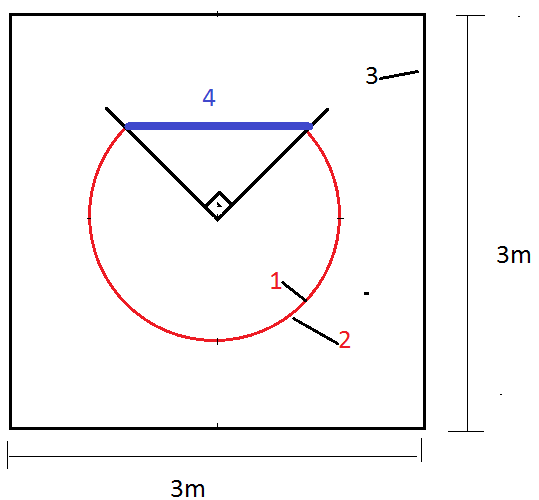
\includegraphics[scale=0.28]{./fig/1.png}
%\caption{\label{fig:1}1} 
\end{center}
\end{figure}

\end{document}